\newcommand{\figTimingArbitration}{%
  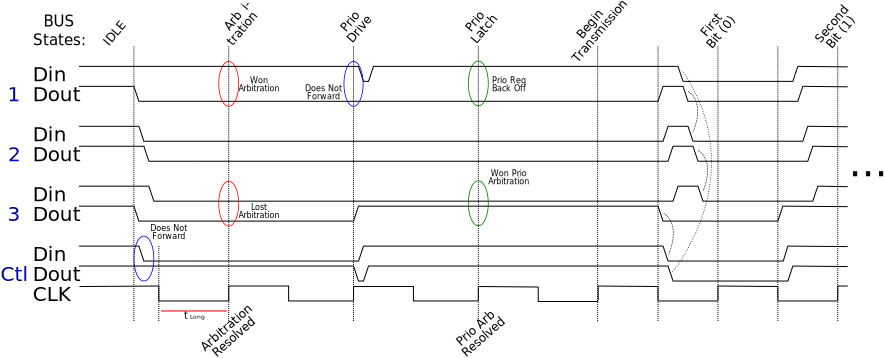
\includegraphics[width=\linewidth]{img/arbitration}
  \caption{
    \bus Arbitration. To begin a transaction, nodes pull down on data.
    Here we show node~1 and node~3 simulataneously requesting the bus.
    Node~1 initially wins arbitration, but node~3 uses the priority
    arbitration cycle to claim the bus. In implementation, nodes may begin
    driving data lines at the Begin~Transmission edge but all subsequent
    data transitions must take place on the falling edge of {\tt CLK}.
  }
  \label{fig:arbitration}
} % End \figTimingArbitration



\newcommand{\figTimingInterrupt}{%
\hspace{-1em}
\noindent\makebox[\textwidth]{%
  \footnotesize
  \begin{tikztimingtable}[timing/wscale=3.0,timing/slope=.3]
    %          10011 EE EE IIIIII SS X110 0II
    CLK In   & CCCCC CC CC CHHHHH HC CCCC CCC\\
    CLK Out  & CCCCC CC CC CHHHHH HC CCCC CCC\\
    Data In  & HHLLH HH HH HCCCCC CH HHHL LHH\\
    Data Out & HHLLH HH HH HCCCCC CH HHHL LHH\\
             & {1D{Data 1}}{2D{Data 0}}{2D{Data 1}}
               {2D{Data 1}}{2D{Data 1}}{6D{Interrupt}}{2D{Switch Role}}
               {2D{Control 1}}{2D{ACK=True}}{2D{Idle}}{1D{\ldots}} \\
    \\
    % TX Node
    CLK In   & CCCCC CC CC CHHHHH HC CCCC CCC\\
    CLK Out  & CCCCC CC LL LLLLLL LL CCCC CCC\\
    Data In  & HHLLH HH HH HCCCCC CH HHHL LHH\\
    Data Out & HHLLH HH HH HCCCCC CH HHHL LHH\\
             & {1D{Data 1}}{2D{Data 0}}{2D{Data 1}}
               {4D{Req Interrupt}}{6D{Interrupt}}{2D{Switch Role}}
               {2D{EoM=True}}{2D{Control 0}}{2D{Idle}}{1D{\ldots}} \\
    \\
    CLK In   & CCCCC CC LL LLLLLL LL CCCC CCC\\
    CLK Out  & CCCCC CC LL LLLLLL LL CCCC CCC\\
    Data In  & HHLLH HH HH HCCCCC CH HHHL LHH\\
    Data Out & HHLLH HH HH HCCCCC CH HHHL LHH\\
             & {1D{Data 1}}{2D{Data 0}}{2D{Data 1}}
               {10D{Interrupt}}{2D{Switch Role}}
               {2D{Control 1}}{2D{Control 0}}{2D{Idle}}{1D{\ldots}} \\
    \\
    % CTL Node
    CLK In   & CCCCC CC LLL LLLLL LL CCCC CCC\\
    CLK Out  & CCCCC CC CCC HHHHH HC CCCC CCC\\
    Data In  & HHLLH HH HHH CCCCC CH HHHL LHH\\
    Data Out & HHLLH HH HHH CCCCC CH HHHL LHH\\
    Int Clk  & CCCCC CC CCC CCCCC CC CCCC CCC\\
             & {1D{Data 1}}{2D{Data 0}}{2D{Data 1}}
               {4D{Enter Interrupt}}{6D{Interrupt}}{2D{Switch Role}}
               {2D{Control 1}}{2D{Control 0}}{2D{Idle}}{1D{\ldots}} \\
  \extracode
    \begin{pgfonlayer}{background}
      \begin{scope}[semithick,dashed]
        \vertlines[color=red]{3,9,...,27}
        \vertlines[color=gray]{6,12,...,15}
        \vertlines[color=blue]{45,51,...,\twidth}
        \vertlines[color=OliveGreen]{48,54,...,\twidth}

        \filldraw[yellow,opacity=.25] (15, 2) rectangle (27, -45);
      \end{scope}
    \end{pgfonlayer}

    \draw[red,thick]    (21,  -2.5) ellipse (1.25 and 4.5);
    \draw[red,thick]    (27,  -2.5) ellipse (1.25 and 4.5);
    \draw[blue,thick]   (45,  -2.5) ellipse (1.25 and 4.5);
    \draw[green,thick]  (45, -26.5) ellipse (1.25 and 4.5);
    \draw[cyan,thick]   (24, -36.5) ellipse (1.25 and 2.5);
    \draw[cyan,semithick,dashed] (24,-44.5) to (24,-33.25); % .25 better dash
    \node at (18, -7.5)  {\huge\color{blue} X};
    \node at (24, -7.5)  {\huge\color{blue} X};
    \node at (18, -31.5) {\huge\color{green} $\checkmark$};
    \node at (24, -31.5) {\huge\color{green} $\checkmark$};

    \begin{scope}
      [font=\bf\sffamily,shift={(-5.5em,-1.5)},anchor=east,color=blue]
      \node [rotate=45] at (  0,   0) {1};
      \node [rotate=45] at (  0, -12) {2 (TX)};
      \node [rotate=45] at (  0, -24) {3};
      \node [rotate=45] at (  0, -36) {Ctl};
    \end{scope}

    \foreach \n [evaluate=\n as \l using int((\n-1)/3)] in {3,6,...,\twidth}
      \draw (\n,-46.5) -- +(0,-.2)
        node [below,inner sep=2pt] {\scalebox{.75}{\footnotesize\l}};
  \end{tikztimingtable}
}
  \caption{
    Detail of the Interrupt entry procedure and control bits. In this example,
    Node~2 is the TX node, thus when it elects to enter Interrupt it is
    already forwarding its data lines. Node~2 decides to enter Interrupt at
    time~4. At time~6 Node~2 suppresses the clock edge, requesting Interrupt.
    The control layer detects this at time~7\protect\footnotemark.  At this
    point the control node begins toggling the {\em data} lines to interrupt
    the bus. After three data pulses, all nodes will enter Interrupt. Two
    control bits are sent, after which the bus returns to Idle.
  }
  \label{fig:interrupt}
} % End \figTimingInterrupt
